\section{连续映射、拓扑空间的连通与道路连通}\label{sec:7.2}

这一节先引进映射的连续及连续映射与同胚映射的概念, 论述它们有关的性质. 在此基础上, 研究了拓扑空间的连通与道路连通性. 还证明了 $(\mathbb{R}^{n}, \mathcal{T}_{\rho_{0}^{n}})$ 中的开集, 其连通、道路连通与折线连通是彼此等价的. 从而对 $(\mathbb{R}^{n}, \mathcal{T}_{\rho_{0}^{n}})$ 中开区域的定义给出了清晰的描述.

\begin{definition}\label{def:7.2.1}
设 $(X, \mathcal{T}_1)$ 与 $(Y, \mathcal{T}_2)$ 为拓扑空间, $f\colon X \to Y$ 为映射, $x_0 \in X$. 如果对 $f(x_0) \in Y$ 的任何开邻域 $V$, 均存在 $x_0$ 的开邻域 $U$, 使得
\[
  f(U) \subset V,
\]
则称 $f$ 在 $x_{0}$ \textbf{连续} (见\cref{fig:7.2.1}). 如果 $f$ 在 $X$ 上的每一点处连续, 则称 $f$ 为 $X$ 上的\textbf{连续映射}或 $f$ 在 $X$ 上是连续的. 如果 $f$ 为一一连续映射, 且 $f^{-1}$ 也连续, 则称 $f$ 为\textbf{拓扑映射}或\textbf{同胚}. 如果 $(X, \mathcal{T}_{1})$ 与 $(Y, \mathcal{T}_{2})$ 之间存在一个同胚, 则称它们为\textbf{同胚的拓扑空间}, 记作 $(X, \mathcal{T}_{1}) \cong (Y, \mathcal{T}_{2})$, 简记为 $X \cong Y$; 否则称为不同胚的拓扑空间, 记作 $(X, \mathcal{T}_{1}) \not\cong (Y, \mathcal{T}_{2})$, 简记为 $X \not\cong Y$.
\end{definition}

\begin{figure}[htbp]
  \centering
  \begin{tikzpicture}[>=latex, scale=1.0]
    % Space X
    \draw[thick] (0, 0) circle (1.3);
    \node at (0, 0.95) {$X$};
    \coordinate (x0) at (0, -0.2);
    \fill[pattern=north east lines, pattern color=black!70] (x0) circle (0.45);
    \draw[dashed, thick] (x0) circle (0.45);
    \fill (x0) circle (1.8pt);
    \node[above=2pt] at (x0) {$U$};
    \node[below=2pt] at (x0) {$x_0$};

    % Arrow f
    \draw[->, thick] (1.7, 0) -- node[above] {$f$} (3.3, 0);

    % Space Y
    \begin{scope}[shift={(5.0, 0)}]
      \draw[thick] (0, 0) circle (1.3);
      \node at (0, 0.95) {$Y$};
      \coordinate (fx0) at (-0.05, -0.15);
      % V neighborhood
      \draw[dashed, thick] (fx0) circle (0.75);
      \node at (0.42, 0.15) {$V$};
      % f(U) neighborhood
      \fill[pattern=north east lines, pattern color=black!70] (fx0) circle (0.4);
      \draw[dashed, thick] (fx0) circle (0.4);
      \fill (fx0) circle (1.8pt);
      \node[below=2pt] at (fx0) {\small $f(x_0)$};
      % pointer to f(U)
      \draw[->, thin] (0.8, -1.1) node[below right=-2pt] {$f(U)$} -- (0.2, -0.35);
    \end{scope}
  \end{tikzpicture}
  \caption{连续映射示意图}\label{fig:7.2.1}
\end{figure}

\begin{example}\label{ex:7.2.1}
(1) 在 $(\mathbb{R}^{n+1}, \mathcal{T}_{\rho_0^{n+1}})$ 中, 半径为 $r_1>0$ 与 $r_2>0$ 的球心都在原点 $0$ 处的 $n$ 维球面 $S^n(r_1)$ 与 $S^n(r_2)$ 是同胚的;

(2) 在 $(\mathbb{R}^{n+1}, \mathcal{T}_{\rho_0^{n+1}})$ 中, $n$ 维椭球面
\[
  X = \left\{(x_1, x_2, \cdots, x_{n+1}) \;\middle|\; x_i \in \mathbb{R}, \; \frac{x_1^2}{a_1^2} + \cdots + \frac{x_{n+1}^2}{a_{n+1}^2} = 1 \right\}
\]
与 $n$ 维单位球面 $S^n = S^n(1)$ 是同胚的.
\end{example}

\begin{proof}
(1) 取 $f\colon S^{n}(r_{1}) \to S^{n}(r_{2})$, $x \mapsto f(x) = \frac{r_{2}}{r_{1}} x$ 即为所需的同胚.

(2) 取 $f\colon X \to S^{n} = S^{n}(1)$, $x \mapsto f(x) = \frac{x}{\|x\|}$ 即为所需的同胚, 其中
\[
  \|x\| = \sqrt{\sum_{i=1}^{n+1} x_{i}^{2}} = \rho_{0}^{n+1}(x, \boldsymbol{0}).
\]
\end{proof}

容易证明关于度量空间中连续性的等价描述:

\begin{theorem}\label{thm:7.2.1}
在度量空间 $(X, \mathcal{T}_{\rho_1})$ 与 $(Y, \mathcal{T}_{\rho_2})$ 中, $f\colon X \to Y$ 为映射, 则以下结论等价:
\begin{enumerate}
  \item $f$ 在 $x_{0}$ 处连续;
  \item $\forall \varepsilon > 0, \exists \delta > 0$, s.t. $f(B(x_0; \delta)) \subset B(f(x_0); \varepsilon)$;
  \item $\forall \varepsilon > 0, \exists \delta > 0$, 当 $x \in X, \rho_{1}(x, x_{0}) < \delta$ 时, 有 $\rho_{2}(f(x), f(x_{0})) < \varepsilon$.
\end{enumerate}
\end{theorem}

\begin{proof}
只需证 (1) $\Rightarrow$ (2). $\forall \varepsilon > 0$, 显然 $V = B(f(x_0); \varepsilon)$ 为 $f(x_0)$ 的开邻域, 由 $f$ 在 $x_0$ 处连续, 故存在 $x_0$ 的开邻域 $U$, 使得 $f(U) \subset V$. 于是, $\exists \delta > 0$, s.t. $B(x_0; \delta) \subset U$. 这就推得 $f(B(x_0; \delta)) \subset f(U) \subset V = B(f(x_0); \varepsilon)$.

(2) $\Rightarrow$ (1): 对 $f(x_{0})$ 的任何开邻域 $V$, 必有 $\varepsilon > 0$, s.t. $B(f(x_{0}); \varepsilon) \subset V$. 由 (2) 知, $\exists \delta > 0$, s.t. $f(U) = f(B(x_{0}; \delta)) \subset B(f(x_{0}); \varepsilon) \subset V$, 其中 $U = B(x_{0}; \delta)$ 为 $x_{0}$ 的开邻域. 根据\cref{def:7.2.1}, $f$ 在 $x_{0}$ 处连续.
\end{proof}

\begin{theorem}\label{thm:7.2.2}
设 $(X, \mathcal{T}_{1})$ 与 $(Y, \mathcal{T}_{2})$ 为拓扑空间, $f\colon X \to Y$ 为映射, 则下面的 (1), (2), (3) 等价, 且它们中任一成立, 可推得 (4) 成立:
\begin{enumerate}
  \item $f$ 为连续映射;
  \item 开集 $V$ 的逆像 $f^{-1}(V) = \{x \mid x \in X, f(x) \in V\}$ 为开集;
  \item 闭集 $F$ 的逆像 $f^{-1}(F) = \{x \mid x \in X, f(x) \in F\}$ 为闭集;
  \item $\forall x \in X, \forall x_{n} \in X$, $\lim\limits_{n \to +\infty} x_{n} = x$ 蕴涵 $\lim\limits_{n \to +\infty} f(x_{n}) = f(x)$.
\end{enumerate}
\end{theorem}

\begin{proof}
(1) $\Rightarrow$ (2): 若 $f^{-1}(V) = \varnothing$, 则它显然为开集. 若 $f^{-1}(V) \neq \varnothing$, 则 $\forall x \in f^{-1}(V), f(x) \in V \subset Y$. 由 $V$ 为开集, $f$ 连续, 故有 $x$ 的开邻域 $U_{x}$, 使得 $f(U_{x}) \subset V$, 即 $x \in U_{x} \subset f^{-1}(V)$. 所以,
\[
  f^{-1}(V) = \bigcup_{x \in f^{-1}(V)} \{x\} \subset \bigcup_{x \in f^{-1}(V)} U_{x} \subset f^{-1}(V),
\]
即
\[
  f^{-1}(V) = \bigcup_{x \in f^{-1}(V)} U_{x}.
\]
根据拓扑定义 (3), $f^{-1}(V)$ 为 $(X, \mathcal{T}_{1})$ 中的开集.

(2) $\Rightarrow$ (1): $\forall x \in X$, 对 $f(x)$ 的任何开邻域 $V$, 由 (2) 知 $f^{-1}(V)$ 为 $x$ 的开邻域, 且 $f(f^{-1}(V)) \subset V$, 所以 $f$ 在 $x$ 处连续. 由 $x$ 的任意性推得 $f$ 为连续映射.

(2) $\Leftrightarrow$ (3): 由 $f^{-1}(Y \setminus B) = X \setminus f^{-1}(B)$ 立即推得.

(1) $\Rightarrow$ (4): 设 $V$ 为 $f(x)$ 的任一开邻域, 因 $f$ 在 $x$ 处连续, 故存在 $x$ 的开邻域 $U$, 使得 $f(U) \subset V$. 由 $\lim\limits_{n \to +\infty} x_n = x \in U$ (开集), 故 $\exists N \in \mathbb{Z}_+$, 当 $n > N$ 时, 有 $x_n \in U$. 于是, $f(x_n) \in f(U) \subset V$. 从而 $\lim\limits_{n \to +\infty} f(x_n) = f(x)$.
\end{proof}

\begin{corollary}\label{cor:7.2.1}
设 $(X, \mathcal{T}_{1})$ 与 $(Y, \mathcal{T}_{2})$ 为拓扑空间, $f\colon X \to Y$ 为映射, 则
\[
  f \text{ 在 } x_{0} \in X \text{ 处连续} \implies \forall x_{n} \in X, \; \lim_{n \to +\infty} x_{n} = x_{0} \implies \lim_{n \to +\infty} f(x_{n}) = f(x_{0}).
\]
\end{corollary}

\begin{proof}
完全仿照\cref{thm:7.2.2}(1) $\Rightarrow$ (4) 的证明.
\end{proof}

关于 $A_{1}$ 空间 (特别是度量空间), 有以下定理:

\begin{theorem}\label{thm:7.2.3}
设 $(X, \mathcal{T}_{1})$ 为 $A_{1}$ 空间 (特别是度量空间), $(Y, \mathcal{T}_{2})$ 为拓扑空间, $f\colon X \to Y$ 为映射, $x_{0} \in X$. 则
\[
  f \text{ 在 } x_{0} \text{ 处连续} \iff \forall x_{n} \in X, \; \lim_{n \to +\infty} x_{n} = x_{0} \implies \lim_{n \to +\infty} f(x_{n}) = f(x_{0}).
\]
\end{theorem}

\begin{proof}
($\Rightarrow$) 由\cref{cor:7.2.1}可得.

($\Leftarrow$) 因为 $(X, \mathcal{T}_{1})$ 为 $A_{1}$ 空间, 故对 $x_{0}$ 有规范可数局部基 $\{U_{n} \mid n \in \mathbb{Z}_{+}\}$. (反证) 假设 $f$ 在 $x_{0}$ 处不连续, 故必有 $f(x_{0})$ 的开邻域 $V$, 对 $x_{0}$ 的任何开邻域 $U$, $f(U) \not\subset V$. 特别对 $x_{0}$ 的开邻域 $U_{n}$, 有 $f(U_{n}) \not\subset V$. 取 $x_{n} \in U_{n}$, s.t. $f(x_{n}) \notin V$. 由 $\{U_{n} \mid n \in \mathbb{Z}_{+}\}$ 为 $x_{0}$ 处的规范可数局部基及点列极限的定义得到 $\lim\limits_{n \to +\infty} x_{n} = x_{0}$. 但 $\lim\limits_{n \to +\infty} f(x_{n}) \neq f(x_{0})$, 这与条件相矛盾.
\end{proof}

\begin{theorem}\label{thm:7.2.4}
设 $\mathbb{R}^n$ 与 $\mathbb{R}^m$ 为通常的 $n$ 维与 $m$ 维 Euclid 拓扑空间, $Y$ 为 $\mathbb{R}^n$ 中的子拓扑空间, 则以下结论等价:
\begin{enumerate}
  \item $f = (f_1, f_2, \cdots, f_m)\colon Y \to \mathbb{R}^m$ 在 $x^0 = (x_1^0, x_2^0, \cdots, x_n^0)$ 连续;
  \item $f_i\colon Y \to \mathbb{R}$ 在 $x^0$ 连续, $i = 1, 2, \cdots, m$.
\end{enumerate}
\end{theorem}

\begin{proof}
从不等式
\[
  |f_{i}(x) - f_{i}(x^{0})| \leqslant \rho_{0}(f(x), f(x^{0})) = \sqrt{\sum_{j=1}^{m} [f_{j}(x) - f_{j}(x^{0})]^{2}} \leqslant \sqrt{m} \max_{1 \leqslant j \leqslant m} |f_{j}(x) - f_{j}(x^{0})|
\]
与连续定义\cref{def:7.2.1}立即推出结论.
\end{proof}

下面将介绍与连续映射密切相关的道路连通这一重要概念.

\begin{definition}\label{def:7.2.2}
设 $(X, \mathcal{T})$ 为拓扑空间, $[0,1]$ 为通常 Euclid 直线 $(\mathbb{R}^{1}, \mathcal{T}_{\rho_0^1})$ 的子拓扑空间. 如果对 $\forall p, q \in X$, 存在连接 $p$ 与 $q$ 的一条道路, 即存在连续映射
\[
  \sigma\colon [0,1] \to X,
\]
使得 $\sigma(0) = p, \sigma(1) = q$, 则称 $(X, \mathcal{T})$ 为\textbf{道路连通的拓扑空间} (见\cref{fig:7.2.2}).
\end{definition}

\begin{figure}[htbp]
  \centering
  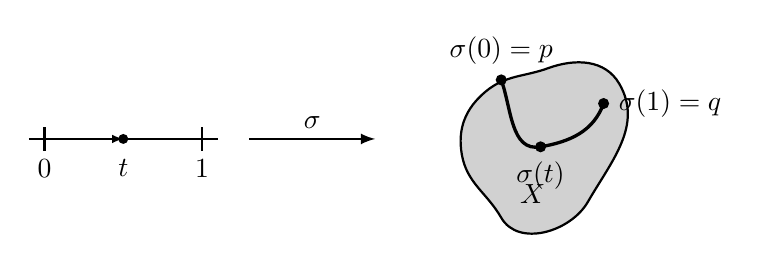
\begin{tikzpicture}[>=latex, scale=1.0]
    % Interval [0, 1]
    \draw[thick] (-0.2, 0) -- (2.2, 0);
    \draw[thick] (0, -0.15) -- (0, 0.15) node[below=8pt] {$0$};
    \draw[thick] (2.0, -0.15) -- (2.0, 0.15) node[below=8pt] {$1$};
    \fill (1.0, 0) circle (1.8pt);
    \draw[->] (0.7, 0) -- (1.0, 0);
    \node[below=4pt] at (1.0, 0) {$t$};

    % Arrow sigma
    \draw[->, thick] (2.6, 0) -- node[above] {$\sigma$} (4.2, 0);

    % Set X
    \begin{scope}[shift={(5.6, 0)}]
      \def\xshape{(0, 0.6) to[out=40, in=-160] (0.8, 0.9)
                  to[out=20, in=120] (1.7, 0.7)
                  to[out=-60, in=60] (1.3, -0.8)
                  to[out=-120, in=-60] (0.2, -1.0)
                  to[out=120, in=-80] (-0.3, -0.2)
                  to[out=100, in=-140] (0, 0.6)}
      \fill[black!18] \xshape;
      \draw[thick] \xshape;
      \node at (0.6, -0.7) {$X$};

      % Curve sigma(t)
      \coordinate (P) at (0.2, 0.75);
      \coordinate (Q) at (1.5, 0.45);
      \draw[very thick] (P) to[out=-70, in=-170] (0.7, -0.1)
                           to[out=10, in=-110] (Q);
      \fill (P) circle (2pt) node[above=2pt] {$\sigma(0)=p$};
      \fill (Q) circle (2pt) node[right=2pt] {$\sigma(1)=q$};
      \coordinate (Pt) at (0.7, -0.1);
      \fill (Pt) circle (2pt);
      \node[below=2pt] at (Pt) {$\sigma(t)$};
    \end{scope}
  \end{tikzpicture}
  \caption{道路连通示意图}\label{fig:7.2.2}
\end{figure}

应该注意的是, 道路指的是连续映射 $\sigma$, 而不是 $\sigma$ 的像 $\sigma([0,1]) = \{\sigma(t) \mid t \in [0,1]\}$.

\begin{example}\label{ex:7.2.2}
设 $X$ 为 $\mathbb{R}^n$ 中的一个凸集, 即 $\forall p, q \in X, \forall t \in [0,1]$, 必有 $(1-t)p + tq \in X$, 则 $X$ 作为通常的 Euclid 空间 $(\mathbb{R}^n, \mathcal{T}_{\rho_0}^n)$ 的子拓扑空间是道路连通的. 事实上, 只需取连接 $p$ 与 $q$ 的道路为 $\sigma\colon [0,1] \to X, \sigma(t) = (1-t)p + tq$ (\cref{fig:7.2.3}).

显然, 直线上的 (开或闭或半开半闭) 区间, 平面上的 (开或闭) 圆片 (椭圆片), $\mathbb{R}^{n} (n \geqslant 3)$ 中的 (开或闭) 球体 (椭球体), 还有 $\mathbb{R}^{n} (n \geqslant 1)$ 本身都是凸集. 因而, 它们都是道路连通的.

考察平面上的集合
\[
  X = [-2, 2] \times [-1, 0] \cup [-2, -1] \times [0, 1] \cup [1, 2] \times [0, 1],
\]
它是道路连通的, 但不是凸集 (\cref{fig:7.2.4}).
\end{example}

\begin{figure}[htbp]
  \centering
  \begin{minipage}[b]{0.45\linewidth}
    \centering
    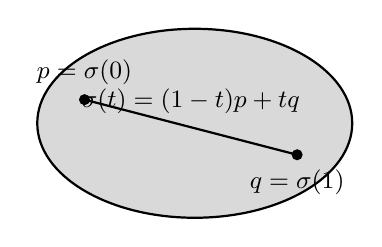
\begin{tikzpicture}[>=latex, scale=1.0]
      % Convex ellipse
      \fill[black!15] (0, 0) ellipse (2.0 and 1.2);
      \draw[thick] (0, 0) ellipse (2.0 and 1.2);

      \coordinate (p) at (-1.4, 0.3);
      \coordinate (q) at (1.3, -0.4);
      \draw[thick] (p) -- node[above=1pt] {\small $\sigma(t)=(1-t)p+tq$} (q);
      \fill (p) circle (2pt) node[above=2pt] {\small $p=\sigma(0)$};
      \fill (q) circle (2pt) node[below=2pt] {\small $q=\sigma(1)$};
    \end{tikzpicture}
    \caption{凸集是道路连通的}\label{fig:7.2.3}
  \end{minipage}\qquad
  \begin{minipage}[b]{0.48\linewidth}
    \centering
    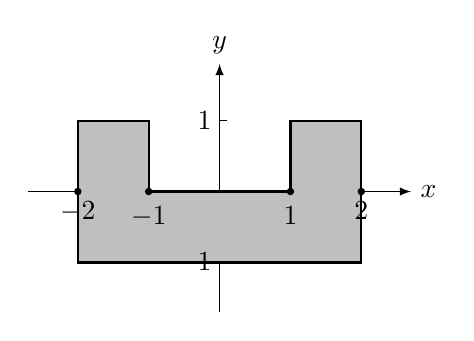
\begin{tikzpicture}[>=latex, scale=0.9]
      % Axes
      \draw[->] (-2.7, 0) -- (2.7, 0) node[right] {$x$};
      \draw[->] (0, -1.7) -- (0, 1.8) node[above] {$y$};
      \node[below left] at (0, 0) {$O$};

      % Set X shaded
      \fill[black!25] (-2, -1) rectangle (2, 0);
      \fill[black!25] (-2, 0) rectangle (-1, 1);
      \fill[black!25] (1, 0) rectangle (2, 1);

      % Boundary of X
      \draw[thick] (-2, 0) -- (-2, 1) -- (-1, 1) -- (-1, 0) -- (1, 0) -- (1, 1) -- (2, 1) -- (2, -1) -- (-2, -1) -- cycle;

      % Ticks & labels
      \draw (0, 1) -- (0.1, 1) node[left=2pt] {$1$};
      \draw (0, -1) -- (0.1, -1) node[left=2pt] {$-1$};
      \fill (-2, 0) circle (1.5pt) node[below] {$-2$};
      \fill (-1, 0) circle (1.5pt) node[below=2pt] {$-1$};
      \fill (1, 0) circle (1.5pt) node[below=2pt] {$1$};
      \fill (2, 0) circle (1.5pt) node[below] {$2$};
    \end{tikzpicture}
    \caption{道路连通但非凸集}\label{fig:7.2.4}
  \end{minipage}
\end{figure}

\begin{definition}\label{def:7.2.3}
设 $(X, \mathcal{T})$ 为拓扑空间, 如果 $X$ 为两个不相交的非空开集的并, 则称 $(X, \mathcal{T})$ 为\textbf{非连通的拓扑空间}, 否则称为\textbf{连通的拓扑空间}.
\end{definition}

易见:
\begin{align*}
  X \text{ 非连通} &\iff X \text{ 为两个不相交的非空闭集的并} \\
  &\iff X \text{ 含有一个非空的真子集, 它既为开集又为闭集}.
\end{align*}

\begin{example}\label{ex:7.2.3}
$[a,b]$ ($a<b, a, b \in \mathbb{R}$) 作为 $(\mathbb{R}^{1}, \mathcal{T}_{\rho_{0}}^{1})$ 的子拓扑空间是连通的.
\end{example}

\begin{proof}
(反证) 假设 $[a,b]$ 非连通, 则 $[a,b] = U \cup V$, $U$ 与 $V$ 为 $[a,b]$ 中不相交的非空开集. 取 $p \in U, q \in V$, 不妨设 $p < q$. 令
\[
  \xi = \sup\{x \mid x \in U \cap [p,q]\}.
\]
由 $U$ 与 $V$ 为开集, 易见 $p < \xi < q$. 再由 $\sup$ 的定义知 $\xi \notin V \cap [p, q]$, 而由 $(\xi, q) \subset V$ 知 $\xi \notin U \cap [p, q]$. 因此,
\[
  \xi \notin (U \cap [p,q]) \cup (V \cap [p,q]) = (U \cup V) \cap [p,q] = [p,q],
\]
这与 $\xi \in [p, q]$ 相矛盾.

类似可证 $(a,b)$, $[a,b)$, $(a,b]$, $(-\infty, a)$, $(-\infty, a]$, $[a, +\infty)$, $(a, +\infty)$, $(-\infty, +\infty)$ 都是连通的.
\end{proof}

\begin{theorem}\label{thm:7.2.5}
拓扑空间 $(X, \mathcal{T})$ 道路连通必连通, 但反之不真.
\end{theorem}

\begin{proof}
(反证) 假设 $(X, \mathcal{T})$ 非连通, 则 $X = U \cup V$, $U$ 与 $V$ 为 $(X, \mathcal{T})$ 中的非空不相交的开集. 取 $p \in U, q \in V$, 显然 $p \neq q$. 因 $(X, \mathcal{T})$ 道路连通, 故存在连接 $p$ 与 $q$ 的道路 $\sigma\colon [0,1] \to X$, 使 $\sigma(0) = p \in U, \sigma(1) = q \in V$. 于是,
\[
  [0,1] = \sigma^{-1}(X) = \sigma^{-1}(U \cup V) = \sigma^{-1}(U) \cup \sigma^{-1}(V),
\]
其中 $0 \in \sigma^{-1}(U), 1 \in \sigma^{-1}(V)$. 由 $\sigma$ 连续知 $\sigma^{-1}(U)$ 与 $\sigma^{-1}(V)$ 为 $[0,1]$ 的不相交的非空开集, 从而 $[0,1]$ 非连通, 这与\cref{ex:7.2.3}中的结论相矛盾.

反之不真, 参阅\cref{ex:7.2.5}与\cref{ex:7.2.6}.
\end{proof}

\cref{thm:7.2.5}与\cref{ex:7.2.2}表明, $(\mathbb{R}^{n}, \mathcal{T}_{\rho_{0}^{n}})$ 中的任何凸集都是道路连通的, 因而也是连通的.

\begin{example}\label{ex:7.2.4}
设 $A$ 为平面 $(\mathbb{R}^2, \mathcal{T}_{\rho_0}^2)$ 中的至多可数集, 则 $\mathbb{R}^2 \setminus A$ 为 $(\mathbb{R}^2, \mathcal{T}_{\rho_0}^2)$ 的道路连通子集, 当然也是连通子集.
\end{example}

\begin{proof}
$\forall p, q \in \mathbb{R}^2 \setminus A, p \neq q$. 作线段 $\overline{pq}$ 的垂直平分线 $l$, 再过 $p, q$ 并以 $\overline{pq}$ 为弦作圆弧, 则必有一条圆弧 $\overset{\frown}{prq} \subset \mathbb{R}^2 \setminus A$ (如\cref{fig:7.2.5}, 因 $A$ 为至多可数集, $l$ 上的点不可数, 故圆弧为不可数集), 它就是 $\mathbb{R}^2 \setminus A$ 中连接 $p$ 与 $q$ 的一条道路, 从而, $\mathbb{R}^2 \setminus A$ 是道路连通的. 再根据\cref{thm:7.2.5}, $\mathbb{R}^2 \setminus A$ 也是连通的.
\end{proof}

\begin{figure}[htbp]
  \centering
  \begin{tikzpicture}[>=latex, scale=1.0]
    % Axes
    \draw[->] (-0.3, 0) -- (4.2, 0) node[right] {$x$};
    \draw[->] (0, -0.3) -- (0, 2.5) node[above] {$y$};
    \node[below left] at (0, 0) {$O$};

    % Points p and q
    \coordinate (p) at (0.4, 0.4);
    \coordinate (q) at (3.5, 1.0);
    \fill (p) circle (2pt) node[below=2pt] {$p$};
    \fill (q) circle (2pt) node[right=2pt] {$q$};

    % Straight line pq (for construction)
    \draw[thick] (p) -- (q);

    % Midpoint and perpendicular bisector l
    \coordinate (m) at ($(p)!0.5!(q)$);
    \draw[thick] (1.3, 2.2) -- (2.3, -0.2) node[right] {$l$};

    % Circular arc prq
    \draw[very thick] (p) to[out=60, in=165] (1.8, 1.6) to[out=-15, in=140] (q);
    \coordinate (r) at (1.8, 1.6);
    \fill (r) circle (2pt) node[above=2pt] {$r$};
  \end{tikzpicture}
  \caption{$\mathbb{R}^2 \setminus A$ 的圆弧道路}\label{fig:7.2.5}
\end{figure}

\begin{theorem}\label{thm:7.2.6}
设 $(X, \mathcal{T})$ 为拓扑空间, $Y$ 为 $(X, \mathcal{T})$ 的连通子集 (即 $Y$ 作为子拓扑空间是连通的), 且 $Y \subset Z \subset \overline{Y}$, 则 $Z$ 也连通. 特别地, $\overline{Y}$ 是连通的.
\end{theorem}

\begin{proof}
(反证) 假设 $Z$ 非连通, 则 $Z = A \cup B$, $A$ 与 $B$ 为 $Z$ 中不相交的非空开集. 因为连通子集 $Y = (Y \cap A) \cup (Y \cap B)$, 而 $Y \cap A$ 与 $Y \cap B$ 为 $Y$ 中的开集. 所以, $Y \cap A = \varnothing$ 或 $Y \cap B = \varnothing$, 即 $Y \subset B$ 或 $Y \subset A$. 不妨设 $Y \subset A$. 由于
\[
  Z \subset \overline{Y} \subset \overline{A},
\]
故
\[
  Z \cap B \subset \overline{A} \cap B = (\overline{A} \cap Z) \cap B = A^{-} \cap B = A \cap B = \varnothing
\]
(其中 $A^{-}$ 为 $A$ 在 $Z$ 中的相对闭包). 因此, $B = Z \cap B = \varnothing$. 这与假设 $B$ 非空相矛盾.
\end{proof}

\begin{theorem}\label{thm:7.2.7}
设 $(X, \mathcal{T}_{1})$ 与 $(Y, \mathcal{T}_{2})$ 都为拓扑空间, $f\colon X \to Y$ 为连续映射.
\begin{enumerate}
  \item 如果 $(X, \mathcal{T}_{1})$ 连通, 则 $f(X)$ 也连通;
  \item 如果 $(X, \mathcal{T}_{1})$ 道路连通, 则 $f(X)$ 也道路连通.
\end{enumerate}
\end{theorem}

\begin{proof}
(1) (反证) 假设 $f(X)$ 非连通, 则 $f(X) = A \cup B$, 其中 $A$ 与 $B$ 为 $f(X)$ 中的非空不相交的开子集. 由 $f$ 连续及\cref{thm:7.2.2}知, $f^{-1}(A)$ 与 $f^{-1}(B)$ 也为 $X$ 的非空不相交的开子集, 且 $X = f^{-1}(A) \cup f^{-1}(B)$, 从而 $X$ 非连通. 这与已知 $X$ 连通相矛盾. 所以, $f(X)$ 也是连通的.

(2) 设 $p, q \in f(X)$, 则 $\exists a, b \in X$, s.t. $f(a) = p, f(b) = q$. 因为 $(X, \mathcal{T}_1)$ 道路连通, 所以有连续映射 $\eta\colon [0, 1] \to X$, 使 $\eta(0) = a, \eta(1) = b$. 于是,
\[
  \sigma = f \circ \eta\colon [0, 1] \to f(X),
\]
\[
  \sigma(0) = f \circ \eta(0) = f(a) = p, \quad \sigma(1) = f \circ \eta(1) = f(b) = q
\]
为 $f(X)$ 中连接 $p$ 与 $q$ 的一条道路, 因此, $f(X)$ 是道路连通的.
\end{proof}

从\cref{thm:7.2.7}可知, 连通与道路连通都是拓扑不变性质.

\begin{example}\label{ex:7.2.5}
设
\[
  A = \left\{(x,y) \;\middle|\; y = \sin\frac{1}{x}, \; 0 < x \leqslant \frac{2}{\pi}\right\} \subset \mathbb{R}^{2}, \quad B = \left\{(0,y) \;\middle|\; -1 \leqslant y \leqslant 1\right\} \subset \mathbb{R}^{2}.
\]
显然, $\overline{A} = A \cup B$.

因为 $A$ 为 $\left(0, \frac{2}{\pi}\right]$ 的连续像, 根据\cref{thm:7.2.7}(2), $A$ 是道路连通的, 当然也是连通的, 再由\cref{thm:7.2.6}, $\overline{A}$ 是连通的, 但 $\overline{A}$ 不是道路连通的. 事实上, 设 $a \in A, b \in B, \sigma\colon [0,1] \to \overline{A}$ 为任一映射, 使得 $\sigma(0) = a, \sigma(1) = b$, 则 $\sigma$ 必不连续 (\cref{fig:7.2.6}).
\end{example}

\begin{proof}
(反证) 假设 $\sigma(t) = (x(t), y(t))$ 连续, 即 $x(t)$ 与 $y(t)$ 均连续. 令
\[
  t_{*} = \inf\{t \in [0,1] \mid \sigma(t) \in B\}.
\]
显然, $0 < t_{*}$. 由 $t_{*}$ 的定义, 存在 $t_{n} \to t_{*}^{+} (n \to +\infty)$, $\sigma(t_{n}) \in B$. 于是,
\[
  \lim_{t \to t_{*}} x(t) = x(t_{*}) = \lim_{n \to +\infty} x(t_{n}) = \lim_{n \to +\infty} 0 = 0,
\]
\[
  y(t_{*}) = \lim_{t \to t_{*}^{-}} y(t) = \lim_{t \to t_{*}^{-}} \sin\frac{1}{x(t)}.
\]
易见, 上式左边 $y(t_{*})$ 为一确定实数, 而右边由于 $\lim\limits_{t \to t_{*}^{-}} x(t) = 0$ 而无极限, 矛盾.
\end{proof}

\begin{figure}[htbp]
  \centering
  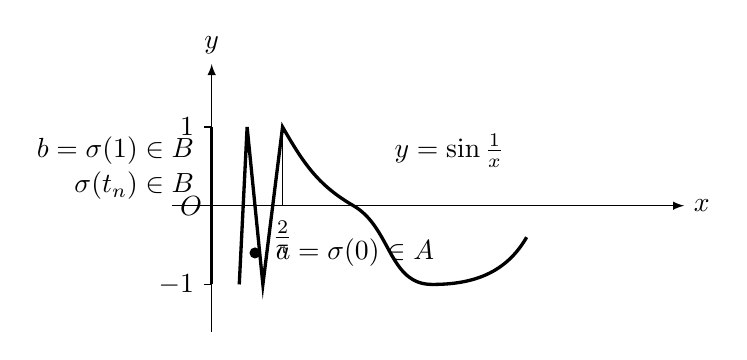
\begin{tikzpicture}[>=latex, scale=1.0]
    % Axes
    \draw[->] (-0.5, 0) -- (6.0, 0) node[right] {$x$};
    \draw[->] (0, -1.6) -- (0, 1.8) node[above] {$y$};
    \node[left] at (0, 0) {$O$};
    \draw (0, 1) -- (-0.1, 1) node[left] {$1$};
    \draw (0, -1) -- (-0.1, -1) node[left] {$-1$};

    % Sine curve: y = sin(1/x)
    \draw[very thick] (0.35, -1.0) -- (0.45, 1.0) -- (0.65, -1.0) -- (0.9, 1.0)
                      to[out=-60, in=150] (1.8, 0)
                      to[out=-30, in=180] (2.8, -1.0)
                      to[out=0, in=-120] (4.0, -0.4);
    
    % Peak at 2/pi
    \coordinate (peak) at (0.9, 1.0);
    \draw[thin] (peak) -- (0.9, 0) node[below=2pt] {$\frac{2}{\pi}$};
    \node[right] at (2.2, 0.7) {$y = \sin \frac{1}{x}$};

    % Limit segment x=0, y in [-1, 1]
    \draw[very thick] (0, -1) -- (0, 1);

    % Points a in A and b in B
    \coordinate (ptA) at (0.55, -0.6);
    \fill (ptA) circle (2pt) node[right=4pt] {$a = \sigma(0) \in A$};

    \node[left] at (-0.1, 0.7) {$b = \sigma(1) \in B$};
    \node[left] at (-0.1, 0.25) {$\sigma(t_n) \in B$};
  \end{tikzpicture}
  \caption{拓扑学家的正弦曲线示意图}\label{fig:7.2.6}
\end{figure}

\begin{example}\label{ex:7.2.6}
设 $\mathbb{R}_{+}^{2} = \{(x,y) \in \mathbb{R}^{2} \mid y > 0\} = (-\infty, +\infty) \times (0, +\infty)$,
\[
  F_{n} = [-n, n] \times \left[\frac{1}{n} - \frac{1}{4n(n+1)}, \; \frac{1}{n} + \frac{1}{4n(n+1)}\right], \quad n = 1, 2, \cdots,
\]
则:
\begin{enumerate}
  \item $G = \mathbb{R}_+^2 \setminus \bigcup\limits_{n=1}^{\infty} F_n$ 为开区域 (连通的开集称为开区域);
  \item $G$ 的闭包 $\overline{G}$ 为 $(\mathbb{R}^{2}, \mathcal{T}_{\rho_{0}}^{2})$ 的连通子集;
  \item $\overline{G}$ 在 $(\mathbb{R}^{2}, \mathcal{T}_{\rho_{0}}^{2})$ 中不是道路连通的.
\end{enumerate}
\end{example}

\begin{proof}
(1) $\forall p \in G$, 显然 $\varepsilon = \rho_{0}^{2}(p, G^{c}) = \inf\limits_{q \in G^{c}} \rho_{0}^{2}(p,q) > 0$, 则以 $p$ 为中心 $\varepsilon$ 为半径的开圆片 $B(p; \varepsilon) \subset G$. 因此, $G$ 为开集.

设 $p, q \in G, p \neq q$, 显然在 $G$ 中存在折线 (由平行于坐标轴的直线段组成) 将 $p$ 与 $q$ 相连接. 因此, $G$ 是折线连通的, 当然是道路连通的. 根据\cref{thm:7.2.5}知, 它也是连通的. 这就证明了 $G$ 为连通的开集, 即 $G$ 为开区域.

(2) 由\cref{thm:7.2.6}推得 $\overline{G}$ 是连通的.

(3) (反证) 假设 $\overline{G}$ 是道路连通的, 则对 $(0,0) \in \overline{G}, (0,2) \in \overline{G}$, 必有连接 $(0,0)$ 与 $(0,2)$ 的一条道路, 即存在连续映射
\[
  \sigma\colon [0,1] \to \overline{G}, \quad \sigma(t) = (x(t), y(t)), \quad \sigma(0) = (0,0), \quad \sigma(1) = (0,2),
\]
其中 $x(t), y(t)$ 均为 $t$ 的连续函数 (\cref{fig:7.2.7}). 由一元连续函数的最值定理, $\exists t_{*} \in [0,1]$, s.t. $|x(t_{*})| = \max\limits_{t \in [0,1]} |x(t)|$. 取 $N \in \mathbb{Z}_{+}$, s.t. $N > |x(t_{*})|$. 由于 $0 < \frac{1}{N} < 2$ 和一元连续函数的介值定理, $\exists t_{**} \in (0,1)$, s.t. $y(t_{**}) = \frac{1}{N}$. 所以
\begin{align*}
  (x(t_{**}), y(t_{**})) &= \left(x(t_{**}), \frac{1}{N}\right) \in \left([-|x(t_{*})|, |x(t_{*})|] \times \left\{\frac{1}{N}\right\}\right) \cap \overline{G} \\
  &\subset \left((-N, N) \times \left\{\frac{1}{N}\right\}\right) \cap \overline{G} = \varnothing,
\end{align*}
矛盾. 从而 $\overline{G}$ 不是道路连通的.
\end{proof}

\begin{figure}[htbp]
  \centering
  \begin{tikzpicture}[>=latex, scale=1.0]
    % Axes
    \draw[->] (-2.5, 0) -- (3.5, 0) node[right] {$x$};
    \draw[->] (0, -0.5) -- (0, 2.6) node[above] {$y$};
    \node[below right] at (0, 0) {$O$};

    % Ticks on x
    \draw (-2, 0) -- (-2, -0.1) node[below] {$-2$};
    \draw (-1, 0) -- (-1, -0.1) node[below] {$-1$};
    \draw (1, 0) -- (1, -0.1) node[below] {$1$};
    \draw (2, 0) -- (2, -0.1) node[below] {$2$};

    % Horizontal strips at heights 1/N, 1/2, 1
    % Height 1/N (black filled strip)
    \fill[black] (-2.5, 0.15) rectangle (2.5, 0.3);
    \draw[thick] (-2.5, 0.15) rectangle (2.65, 0.3);
    \draw (0, 0.22) -- (-0.1, 0.22) node[left=1pt] {$\frac{1}{N}$};

    % Height 1/2 (shaded strip)
    \fill[black!30] (-2, 0.45) rectangle (2.2, 0.6);
    \draw[thick] (-2, 0.45) rectangle (2.2, 0.6);
    \draw (0, 0.52) -- (-0.1, 0.52) node[left=1pt] {$\frac{1}{2}$};

    % Height 1 (hatched strip)
    \fill[pattern=north east lines, pattern color=black!70] (-1, 0.9) rectangle (1.2, 1.2);
    \draw[thick] (-1, 0.9) rectangle (1.2, 1.2);
    \draw (0, 1.05) -- (-0.1, 1.05) node[left=1pt] {$1$};

    \draw (0, 2) -- (-0.1, 2) node[left=1pt] {$2$};

    % Path from y=2 descending to strip 1/N
    \coordinate (start) at (0, 2.0);
    \draw[very thick, ->] (start) to[out=0, in=120] (0.8, 1.6)
                                 to[out=-60, in=170] (1.8, 1.4)
                                 to[out=-10, in=90] (2.4, 0.45);
    \draw[very thick, ->] (2.4, 0.45) to[out=-90, in=0] (1.5, 0.1)
                                     to[out=180, in=-20] (0, 0);

    % Pointer label
    \draw[<-] (2.45, 0.25) -- (2.8, 0.5) node[right] {$\left(x(t_{**}), \frac{1}{N}\right)$};
    \draw[<-] (2.45, 0.4) -- (2.8, 0.9) node[right] {$(x(t_*), y(t_*))$};
    \draw (2.45, 0.1) -- (2.45, -0.1) node[below] {$|x(t_*)|$};
  \end{tikzpicture}
  \caption{闭梳空间连通但非道路连通示意图}\label{fig:7.2.7}
\end{figure}

\begin{theorem}\label{thm:7.2.8}
设 $U$ 为 $(\mathbb{R}^{n}, \mathcal{T}_{\rho_{0}^{n}})$ 中的开集, 则以下结论等价:
\begin{enumerate}
  \item $U$ 折线连通;
  \item $U$ 道路连通;
  \item $U$ 连通.
\end{enumerate}
\end{theorem}

\begin{proof}
(1) $\Rightarrow$ (2): 因为折线道路是特殊的道路, 所以 $U$ 折线连通必为道路连通.

(2) $\Rightarrow$ (3): 由\cref{thm:7.2.5}即得结论.

(3) $\Rightarrow$ (1): 设 $U_x = \{ y \mid y \in U, \text{存在 } U \text{ 中连接 } x \text{ 与 } y \text{ 的折线} \}$, 则 $U_x$ 为 $(\mathbb{R}^n, \mathcal{T}_{\rho_0^n})$ 中的开集. 事实上, $\forall p \in U_x \subset U$, 由 $U$ 为开集, 存在 $p$ 的开球邻域 $B(p; \varepsilon) \subset U$, 而 $\forall q \in B(p; \varepsilon)$, 有直线段 $\overline{pq}$ 连接 $p$ 与 $q$. 因此, 在 $U$ 中有折线将 $x$ 与 $q$ 相连, 即 $q \in U_x$, $B(p; \varepsilon) \subset U_x$, 故 $U_x$ 为开集 (\cref{fig:7.2.8}).

易见, $U_{x_{1}}$ 与 $U_{x_{2}}$ 或者不相交, 或者重合. 并且,
\[
  U = U_{x} \cup \left(\bigcup_{y \in U \setminus U_{x}} U_{y}\right).
\]
由题设 $U$ 连通及 $U_x$ 非空 (因 $x \in U_x$) 可知 $\bigcup\limits_{y \in U \setminus U_x} U_y = \varnothing$, 从而 $U = U_x$, 明显地, $U$ 是折线连通的.
\end{proof}

\begin{figure}[htbp]
  \centering
  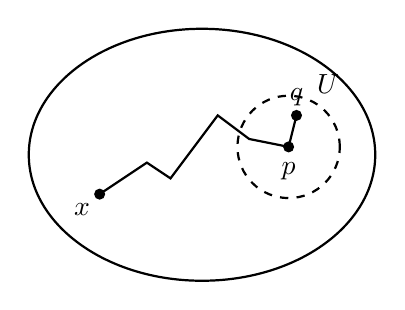
\begin{tikzpicture}[>=latex, scale=1.0]
    % Boundary of U (smooth oval)
    \draw[thick] (0, 0) circle [x radius=2.2, y radius=1.6];
    \node at (1.6, 0.9) {$U$};

    % Points x and p
    \coordinate (x) at (-1.3, -0.5);
    \coordinate (p) at (1.1, 0.1);
    \fill (x) circle (2pt) node[below left] {$x$};

    % Broken line path from x to p
    \coordinate (v1) at (-0.7, -0.1);
    \coordinate (v2) at (-0.4, -0.3);
    \coordinate (v3) at (0.2, 0.5);
    \coordinate (v4) at (0.6, 0.2);
    \draw[thick] (x) -- (v1) -- (v2) -- (v3) -- (v4) -- (p);

    % Neighborhood B(p; eps)
    \draw[dashed, thick] (p) circle (0.65);
    \fill (p) circle (2pt) node[below=2pt] {$p$};

    % Point q in B(p; eps)
    \coordinate (q) at (1.2, 0.5);
    \fill (q) circle (2pt) node[above] {$q$};
    \draw[thick] (p) -- (q);
  \end{tikzpicture}
  \caption{开集 $U$ 中的折线连通}\label{fig:7.2.8}
\end{figure}


\begin{exblock}{练习题 7.2}

  \item 设 $x^{0} \in \mathbb{R}^{n}$, 证明: $(\mathbb{R}^{n}, \mathcal{T}_{\rho_{0}^{n}})$ 中开球 $B(x^{0}; \delta)$ 为凸开集, 因而为开区域.

  \item 设 $A \subset \mathbb{R}^n$, 如果 $A$ 既为开集又为闭集, 证明: $A = \varnothing$ 或者 $A = \mathbb{R}^n$.

  \item 应用反证法及\cref{ex:7.2.3}证明 $(\mathbb{R}^{n}, \mathcal{T}_{\rho_{0}^{n}})$ 是连通的.

  \item 设 $(X, \mathcal{T})$ 连通, $\mathcal{T}' \subset \mathcal{T}$ 为 $X$ 的拓扑, 则 $(X, \mathcal{T}')$ 也是连通空间. 上述``连通''改为``道路连通''结论如何? 并说明理由.

  \item 设 $A$ 为拓扑空间 $(X, \mathcal{T})$ 的连通子集, $B$ 为 $(X, \mathcal{T})$ 的既开又闭的子集, 如果 $A \cap B \neq \varnothing$, 则 $A \subset B$.

  \item 设 $Y$ 为拓扑空间 $(X, \mathcal{T})$ 的连通子集, $Z$ 为 $X$ 的子集. 如果 $Y \cap \overline{Z} \neq \varnothing, Y \cap \overline{Z}^c \neq \varnothing$, 证明: $Y \cap \partial Z \neq \varnothing$.

  \item 设 $A$ 为连通空间 $(X, \mathcal{T})$ 的非空真子集. 证明: $\partial A \neq \varnothing$.

  \item 证明: $(\mathbb{R}^{2}, \mathcal{T}_{\rho_{0}}^{2})$ 上所有至少有一个坐标为有理数的点构成的集合是一个道路连通子集.

  \item 设 $Y$ 是拓扑空间 $(X, \mathcal{T})$ 的一个连通子集. 证明: 如果 $A$ 与 $B$ 是 $(X, \mathcal{T})$ 的两个无交开集 (闭集) 使得 $Y \subset A \cup B$, 则或者 $Y \subset A$ 或者 $Y \subset B$.

  \item 证明:
  \begin{enumerate}
    \item 从拓扑空间到平庸拓扑空间的任何映射都为连续映射;
    \item 从离散拓扑空间到拓扑空间的任何映射都为连续映射.
  \end{enumerate}

  \item 证明: $n$ 维 Euclid 空间 $(\mathbb{R}^{n}, \mathcal{T}_{\rho_{0}}^{n})$ ($n \geqslant 2$) 与 $(\mathbb{R}^{1}, \mathcal{T}_{\rho_{0}}^{1})$ 不同胚.

  \item 设连续函数 $f\colon \mathbb{R}^n \to \mathbb{R}^1$ 既取正值又取负值. 证明: 集合 $E = \{x \in \mathbb{R}^n \mid f(x) \neq 0\}$ 为非连通集.
\end{exblock}

\begin{exblock}{思考题 7.2}
  \item 设 $(X, \mathcal{T})$ 为拓扑空间. 证明: $(X, \mathcal{T})$ 非连通 $\iff X$ 中存在两个子集 $A$ 与 $B$ 是隔离的, 即

  \[
    (A \cap \overline{B}) \cup (\overline{A} \cap B) = \varnothing.
  \]

  \item 设 $Y, Z$ 都是拓扑空间 $(X, \mathcal{T})$ 的子集, 其中 $Y$ 是连通的. 证明: 如果 $Z \cap Y \neq \varnothing$ 与 $Z \cap Y^c \neq \varnothing$, 则 $Z \cap \partial Y \neq \varnothing$.

  \item 设 $Y$ 为拓扑空间 $(X, \mathcal{T})$ 的一个子集. 证明: $\overline{Y}$ 为 $(X, \mathcal{T})$ 的一个非连通子集 $\iff X$ 中存在两个非空集合 $A$ 与 $B$ 使得 $Y \subset A \cup B$, $\overline{A} \cap \overline{B} = \varnothing$, $Y \cap A \neq \varnothing$ 与 $Y \cap B \neq \varnothing$ 成立.

  \item 在 Euclid 平面 $(\mathbb{R}^{2}, \mathcal{T}_{\rho_{0}}^{2})$ 中, 令
  \[
    L_{\frac{1}{n}} = \left\{(x,y) \;\middle|\; x - \frac{1}{n}y = 0\right\} \subset \mathbb{R}^{2}, \quad n = 1, 2, \cdots,
  \]
  \[
    L_{0} = \{(0,y) \mid y \in \mathbb{R}\} \subset \mathbb{R}^{2}.
  \]
  证明: $\forall A \subset L_{0}$, 子集 $A \cup \left(\bigcup\limits_{n=1}^{\infty} L_{\frac{1}{n}}\right)$ 是连通的. 它是道路连通的吗?

  \item 设 $A$ 为单位球面 $S^{n} (n \geqslant 2)$ 的一个至多可数的子集. 证明: $S^{n} \setminus A$ 是道路连通的.

  \item 证明: $n$ 维 Euclid 空间 $\mathbb{R}^n (n \geqslant 2)$ (或 $n$ 维单位球面 $S^n (n \geqslant 1)$) 不能嵌入到实数空间 $\mathbb{R}^1$ 中去, 即不存在同胚 $f\colon \mathbb{R}^n \to f(\mathbb{R}^n) \subset \mathbb{R}^1$ (或 $f\colon S^n \to f(S^n) \subset \mathbb{R}^1$).

  \item (\textbf{粘结引理}) 设 $A$ 与 $B$ 为拓扑空间 $(X, \mathcal{T}_{1})$ 中的两个开集 (闭集), 并且 $X = A \cup B$. 又设 $(Y, \mathcal{T}_{2})$ 也为拓扑空间, $f_{1}\colon A \to Y$ 与 $f_{2}\colon B \to Y$ 都为连续映射, 且满足:
  \[
    f_{1}\big|_{A \cap B} = f_{2}\big|_{A \cap B}.
  \]
  则
  \[
    f\colon X \to Y, \quad x \mapsto f(x) = \begin{cases}
      f_{1}(x), & x \in A, \\
      f_{2}(x), & x \in B
    \end{cases}
  \]
  为一个连续映射.

  \item 设 $A$ 与 $B$ 为 $(\mathbb{R}^{n}, \mathcal{T}_{\rho_{0}^{n}})$ 中两个不相交的闭集. 证明: 存在一个连续函数 $f\colon \mathbb{R}^{n} \to \mathbb{R}^{1}$, 使得
  \[
    f\big|_{A} \equiv 1, \quad f\big|_{B} \equiv 0.
  \]
  \textit{提示}: 令 $f(x) = \frac{\rho(x, B)}{\rho(x, A) + \rho(x, B)}$, 其中 $\rho(x, A) = \inf\limits_{y \in A} \rho(x, y)$.

  \item 设 $(X,\mathcal{T}_{1})$ 与 $(Y,\mathcal{T}_{2})$ 都为拓扑空间, $f\colon X \to Y$ 为映射. 证明:
  \[
    f \text{ 为连续映射} \iff \forall A \subset X, \; f(\overline{A}) \subset \overline{f(A)}.
  \]

  \item 举出连续函数 $f\colon \mathbb{R}^1 \to \mathbb{R}^1$ 及 $A \subset \mathbb{R}^1$, 使 $f(\overline{A}) \subsetneq \overline{f(A)}$.
\end{exblock}